\chapter{Discussion and conclusions}


\tab This chapter presents the results of the three analyses, performed on the selected projects (\ref{table:1}). The purpose is to answer the three research questions outlined in Chapter 1.2.

\textit{\textbf{Question 1}} . How the number of source files changed in a commit can influence the logical dependencies of the system and the overlapping rates with the structural dependencies.\\
\tab Based on the results presented in tables \ref{table:5} and \ref{table:6}, from chapter Experimental Results, the number of changed files taken into consideration has an important influence over the overall rates of the logical and structural dependencies overlaps. If no threshold is set for the number of files then we can affirm that a significant number of structural dependencies are also logical. In table \ref{table:5} we have obtained an overlap of structural and logical dependencies of 60,4\% which is with 40,7\% more than if consider only commits with less then 5 source code files changed per commit (Figure \ref{fig:figvenn}) and with 29,2\% more if consider only commits with more then 5 and less then 20 source code files changed per commit.
\begin{figure}[h]
\centering
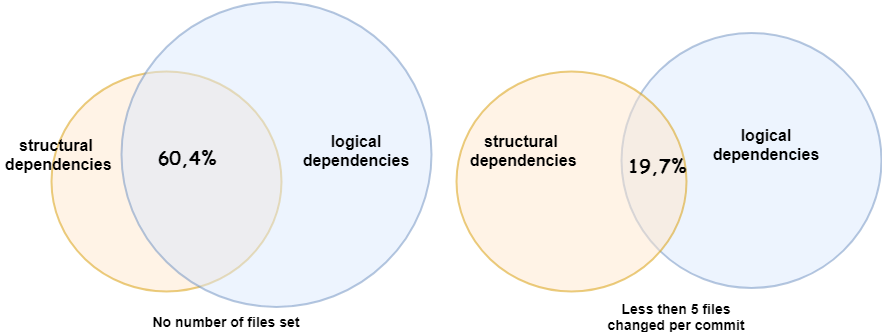
\includegraphics[scale=0.5]{fig4.png}
\caption{Venn diagrams of the overlapping rates with comments taken into consideration as change}
\label{fig:figvenn}
\end{figure}


\textit{\textbf{Question 2}}. Considering comments can lead to additional logical dependencies ? How many logical dependencies are introduced by considering comment changes as valid changes and in what percentage this can influence the final result ?\\

\tab Table \ref{table:comm} illustrates the percentages rates extracted from tables \ref{table:5} and \ref{table:6} from chapter Experimental Results. As it was specified in the tables description , the percentages rates are the number of structural and logical dependencies overlaps, reported to the total number of structural dependencies. How it can be seen, the overlapping rates are also influenced by the comments filtering but in a small percentage. The rates are with aprox 3\% lower if comments are not taken into consideration as a change. (Figure \ref{fig:figvenn2})


\begin{table}
  \centering
  \begin{tabular}{@{}c||cc@{}}
    \toprule
       Category & With comments & Without comments  \\
    \midrule
less 5	&	19,7\% &	18,9\%	\\
more 5 less 20	&	31,19\% &	28,7\%\\
more 20	&	31,47\%	&	29,43\%\\
total & 60,4\% &57,28\% \\
    \bottomrule
  \end{tabular}
  \caption{Average percentages rates with and without considering comments as valid changes.}
   \label{table:comm}
\end{table}

\begin{figure}[h]
\centering
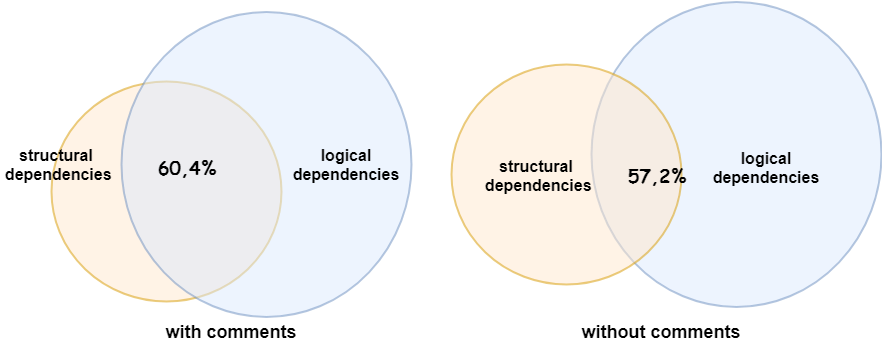
\includegraphics[scale=0.5]{figvenn2.png}
\caption{Venn diagrams of the overlapping rates with comments and without comments taken into consideration.}
\label{fig:figvenn2}
\end{figure}



\textit{\textbf{Question 3}}. One occurrence of a logical dependency is enough to consider it as valid ? If we consider only logical dependencies with more then one occurrence as valid, the results are influenced in a significant way ?\\

\tab Table \ref{table:10} and \ref{table:11} from chapter Experimental Results,  illustrates results in percentages, reported to the structural dependencies, of the analysis for all the systems when logical dependencies where build with/ without comments taken into consideration as change and multiple occurences of logical dependencies taken into consideration as valid dependencies. Based on the experimental results averages \ref{table:14} , we can affirm that the results are with approx 50\% lower after filtering \ref{table:comm} . This indicates that a lot of logical dependencies are the result of a single commit in which the two elements of the dependency where changed together. \\ If we look at the average rates of projects 13 , 15 , 16 , 18 we can observe that the difference is much smaller (15-20\%), the only thing that those projects have in common is the size and the number of commits compared to the other ones from the list, the size and the number of commits of the projects mentioned above are relatively big. \\ This can lead to the conclusion that, if the project studied has a relatively small amount of commits ( Project ID 8.), the probablilty to find multiple updates of the same classes in the same time can be small, so filtering after the number of occurences can lead to filtering all the logical dependencies extracted. (Figure \ref{fig:figvenn3})

\begin{table}
  \centering
  \begin{tabular}{@{}c||cc@{}}
    \toprule
       Category & With comments & Without comments  \\
    \midrule
less 5	&	9,09\% &	8,67\%	\\
more 5 less 20	&	15,87\% &	13,29\%\\
more 20	&	18,8\%	&	16,52\%\\
total &39,1\% & 35,38\% \\
    \bottomrule
  \end{tabular}
  \caption{Overall percentages rates by filtering the logical dependencies occurrences. }
   \label{table:14}
\end{table}


\begin{figure}[h]
\centering
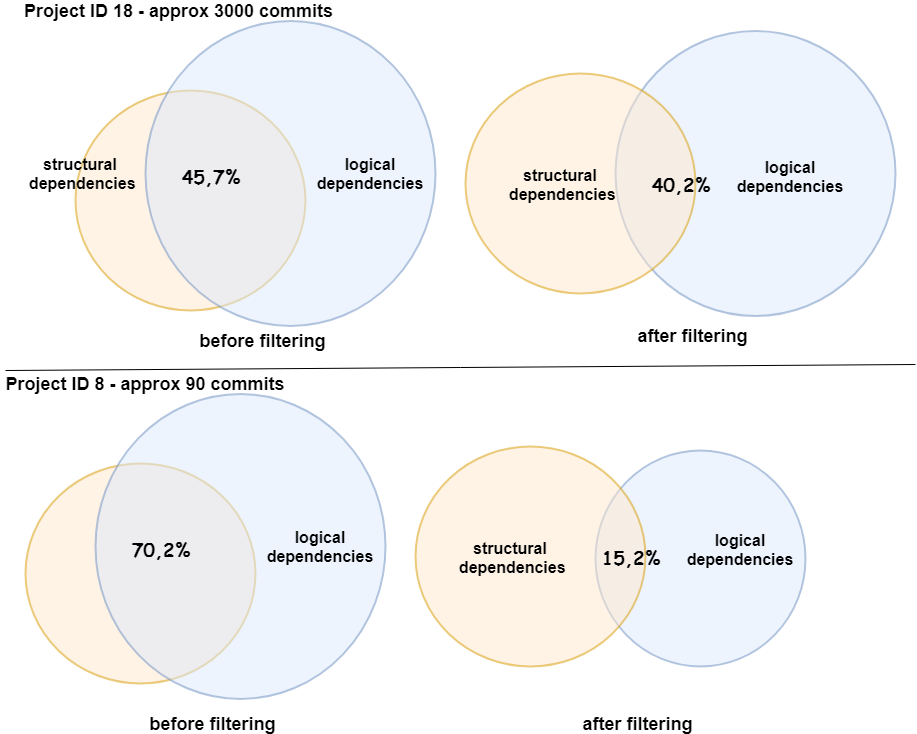
\includegraphics[scale=0.5]{figvenn3.png}
\caption{Impact of logical dependencies occurrences filtering on projects with different sizes.}
\label{fig:figvenn3}
\end{figure}


As a conclusion, it results that large number of structural dependencies are doubled by logical or not, this number is particularly influenced by the number of files that participate in a commit that taken into consideration. It also results that taken or not comments as change, the final results are not influenced in a big percentage. \\ 
\tab In this research work we have tried to identify methods to acquire the most relevant logical dependencies from the system so that can be used in the future for architectural reconstruction, that is currently based only on the information provided by structural dependencies.
\tab For future work, we will investigate the cause for the large number of logical dependencies which are not overlapping with structural dependencies. As we can see in tables \ref{table:ldol1} and \ref{table:ldol2}, where the percentages are reported to the logical dependencies, only a small amount (aprox 10\%) of logical dependencies are also structural .\\ In this work we have been extracted structural dependencies from the last revision of the system but logical dependencies from all the revisions of the system. We will study also structural dependencies from all the revisions of the system since some logical dependencies may have been also structural on previos revisions of the system but not in the current one. If we take into consideration also structural dependencies from previous revisions then the overlapping rate between logical and structural dependencies will probably increase.\\

